\documentclass[10pt,twocolumn,letterpaper]{article}

\usepackage{cvpr}
\usepackage{times}
\usepackage{epsfig}
\usepackage{graphicx}
\usepackage{cite}
\usepackage{amsmath}
\usepackage{amssymb}

% Include other packages here, before hyperref.

% If you comment hyperref and then uncomment it, you should delete
% egpaper.aux before re-running latex.  (Or just hit 'q' on the first latex
% run, let it finish, and you should be clear).
\usepackage[breaklinks=true,bookmarks=false]{hyperref}

\cvprfinalcopy % *** Uncomment this line for the final submission

\def\cvprPaperID{****} % *** Enter the CVPR Paper ID here
\def\httilde{\mbox{\tt\raisebox{-.5ex}{\symbol{126}}}}

% Pages are numbered in submission mode, and unnumbered in camera-ready
%\ifcvprfinal\pagestyle{empty}\fi
\setcounter{page}{2571}
\begin{document}

%%%%%%%%% TITLE
\title{	CNN Based Image Classification}

\author{Xiaoling Long\\
SIST\\
ShanghaiTech Univ.\\
{\tt\small longxl@shanghaitech.edu.cn}
% For a paper whose authors are all at the same institution,
% omit the following lines up until the closing ``}''.
% Additional authors and addresses can be added with ``\and'',
% just like the second author.
% To save space, use either the email address or home page, not both
\and
Hongyu Chen\\
SIST\\
ShanghaiTech Univ.\\
{\tt\small chenhy3@shanghaitech.edu.cn}
\and
Second Author\\
SIST\\
ShanghaiTech Univ.\\
{\tt\small secondauthor@i2.org}
}


\maketitle
%\thispagestyle{empty}

%%%%%%%%% ABSTRACT
\begin{abstract}
   The ABSTRACT is to be in fully-justified italicized text, at the top
   of the left-hand column, below the author and affiliation
   information. Use the word ``Abstract'' as the title, in 12-point
   Times, boldface type, centered relative to the column, initially
   capitalized. The abstract is to be in 10-point, single-spaced type.
   Leave two blank lines after the Abstract, then begin the main text.
   Look at previous CVPR abstracts to get a feel for style and length.
\end{abstract}

%%%%%%%%% BODY TEXT
\section{Introduction}
Image classification is a fundamental challenge in computer vision\cite{felzenszwalb2013visual}. Consider the problem of detecting objects from a category, such as people or cars, in static images. This is a difficult problem because objects in each category can vary greatly in appearance. Variations arise from changes in illumination, viewpoint, and intra-class variability of shape and other visual properties among object instances. For example, people wear different clothes and take a variety of poses while cars come in various shapes and colors.Classification   between   the   objects   is   easy   task   for  humans  but  it  has  proved  to  be  a  complex  problem for machines.Image classification refers to the labeling of images into one of a number of predefined categories.
Image classification is an important and challenging task in various application domains, including biomedical imaging, biometry, video surveillance, vehicle navigation, industrial visual inspection, robot navigation, and remote sensing \cite{kamavisdar2013survey}.

Image classification uses both supervised and unsupervised 
Traditional  methods  of  computer  vision  and  machine
learning cannot match human performance on tasks such
as the recognition of handwritten digits or traffic signs.\cite{ciregancolumn}

Non‐parametric  classifiers  such  as  decision tree   classifier,  neural   network,   SVM   classifier and knowledge based classification are also very common in image classification. 

Disadvantages about the deep learning.For the deep learning based algorithm required the ability of labeled samples for training. The collection of labeled data is a time consuming process as well as costly. 


%-------------------------------------------------------------------------
%\section{CNN Part}

\section{CNN Based Image classification}

\par
The ImageNet Large Scale Visual Recognition Challenge(ILSRC) is a benchmark in object category classification and detection on $1000$-classes and millions of images. After AlexNet achieved hugu success in ILSRC-2012, there are various variations of AlexNet\cite{krizhevsky2012imagenet} and many other types of ConvNet for image classification. Since that, ConvNet is widely used for image classification. \cite{aloysius2017review} illustrate beriefly what is ConvNet, the components of ConvNet, the activation function in ConvNet, from LeNet to ResNet bunch of successful ConvNet and some open issues on CNN based image classification.

\par
AlexNet\cite{krizhevsky2012imagenet} brought Convolutional neural network into ILSRC. In this implementation, it contains 8 layers \- 5 convolutional and 3 fully-conneted. The main features of this network's architecture are ReLU\cite{nair2010rectified} as activation function, overlapping pooling and skills for reducing overfitting. Based on ReLU and overlapping pooling, the network err rate has more or less reduction, and ReLU network learn several times faster than other saturating acitvation function such as tanh neurons network. Overfitting is common issue for machine learning, it uses data augmentation and dropout to avoid overfit. Dropout is a skill to reduce argument or increase hypothesis. There are many discuss about this. As to data augmentation, it enlarge the dataset by cropping $224\times 224$ patched from the original image as well as these patchs' horizontal refliction. At the end averaging the predications as final socre.
\par
\cite{donahue2014decaf} explored the generalization ability of ConvNet features, releasing DeCAF. Traditional image classifition pipeline is extracting feature, building bag of feature then put into classifier. \cite{zeiler2011adaptive} propose a CNN based feature extractor. This is an unsurpervising learning ConvNet or in other words, input image is also the kind of ground truth. After feature extracting, the final result can classify by any classifier. This strategy is used as a tool for visualizing and undestanding how ConvNet works \cite{zeiler2014visualizing}.ConvNet have an impressive classification performance. However there is no clear understanding for why this work. \cite{zeiler2014visualizing} propose a architecture for visualizing and undestanding how ConvNet works.
\par
OverFeat\cite{sermanet2013overfeat} is a integrated recognition, localization and detection. This network uses CNN extract feature from image and then perform classification and localization and detection. Multi-scale classification brought up in \cite{sermanet2013overfeat} to increase accuracy.
\par
``Networ In Network"\cite{lin2013network} propsed a new deep network structure. Different from conventional convolution layer, it brings up a new Mlpconv layer. This Mlpconv layer consist of sliding multilayer perceptron(MLP) window. In stead of fully-connected layer at the top of network, global average pooling is used to produce the resulting vector fed directly into the softmax layer. Verified by experiments, this NIN structure indeed works well on some benchmark datasets, and global average pooling can be regarded as regularizer. THis glolbal average pooling has no parameter. This stratety is used widely afterwards. $1\times 1$ convolution conception proposed in \cite{lin2013network} is used in GoogLeNet for dimension reduction.

\par
AlexNet make a great success in image classification. Afterwards many various Network appear. GoogLeNet\cite{szegedy2015going} proposed by google is a new level of oganization in the form of the `` Inception module". This is a multi-scale arcthitecture. With the limitation of computational resource, it perform a $1\times 1 $ convolution to dimension reduction. Auxiliary classifier is also a brilliant strategy.This smart design makes a great success in ILSRC-2014. At the same time, the widely used ConvNet architecture VGGNet\cite{simonyan2014very}  won the first place in \textit{Classification $+$ Localization competition}. It adds the number of layers up to $16-19$. Instead of $7\times 7$ convolution filter in \cite{simonyan2014very}, it uses $3\times 3$ as convolution filter. After multiple layers, it can get similar effect as $7\times 7 $ one. This design significantly reduces the parameters, and then reduces the overfitting. It also means the number of layers significantly increases. Altering convolutional layers and poolint layer became a common used Network architecture.
\par
As the depth of ConvNet increasing, training gets more and more difficult. The training of very deep network becomes a open issue in CNN. Highway Networks\cite{srivastava2015highway, srivastava2015training} propose \textit{information highways} which allow unimpeded information flow across several layers. The \textit{transform gate} $T(x, W_{T})$ and the \textit{carry gate} $C(x, W_{C})$ proposed for decided how much flow pass through to output. The new model given by
\begin{equation}
  y_{output} = H(x, W_{H})\cdot T(x, W_{T}) + x\cdot C(x, W_{C})
\end{equation}
For simplicty, \cite{he2016deep} set $C = 1 - T$. This design make training hundreds of layers be possible and the err rate just has slightly increase. This architecture promote the success of ResNet \cite{he2016deep}. ResNet has similar structure as deep plain network stacked by dozens of convolution layers followed by global pooling layer and $1$ fully-connected layer. except shortcup connection. This design has a residual representation which called deep residual learning. This archicture keeps parameter less than VGG-19 model even the network has $152$ layers. This smart design make ResNet won first place in ILSRC-15.

There are several works based on region based image classification.Such as \cite{girshick2015fast},\cite{DSDFGVFB}\cite{uijlings2013selective},\cite{alexe2012measuring}. Region based methods are computationally expensively.


R-CNN and fast R-CNN is regioned based convolutional network method for object detection and image classification. In\cite{DSDFGVFB},they use the selective search to select those propose regions. Features are extracted from each proposal region. Then a SVM classifier is used for the category classification. This kind of algorithm need a  lot of time to process each image.  About $2000$ regions are proposed from each image where there maybe several objects in the image. 


Compared to R-CNN\cite{DSDFGVFB}, Fast R-CNN\cite{girshick2015fast} employs several innovations to improve training and testing speed while also increasing detection accuracy. the fast R-CNN has several advantages: (1) higher detection quality  than  R-CNN ,(2) using  a multi task loss ,predict the object and its confidence. No disk storage is required for additional feature catching.The computation is shared during training. Fast achieves a near real time rates uses a very deep network.

Proposal based image classification also contains some great work. Such as \cite{ren2017faster}\cite{redmon2016you}\cite{Redmon2016YOLO9000}\cite{yolov3}.



Faster R-CNN\cite{ren2017faster} is another convolutional network which based on the region proposal methods. In \cite{ren2017faster},The author show that an algorithmic change computing proposals with a deep convolutional neural network leads to an elegant and effective solution where proposal computation is nearly cost-free given the detection network’s computation. They removed the select search algorithm replaced by a region proposal network.
The high quality proposal is used by the Fast R-CNN network for detection and classification. For the very deep VGG-16 model the detection system has a frame rate of 5fps (including all steps) on a GPU, while achieving state-of-the-art object detection accuracy.


Fast and Faster R-CNN focus on speeding up the R-CNN framework by sharing computation and using neural networks to propose regions instead
of Selective Search. While they offer speed and accuracy improvements over R-CNN, both still fall short of real-time performance.
Fast R-CNN speeds up the classification stage of R-CNN but it still relies on selective search which can take around 2 seconds per image to generate bounding box proposals.


In \cite{redmon2016you}, the author achieves a real time detection and classification in $45$  frames per second. A smaller version of their network can be achieved by $ 155$ frames per second. The problem is view as a regression task. The output of the net contains five parameters. $(x,y,w,h,confidence)$ where $x,y,w,h$ means x location , y  location, the width and the height of the target, the probabilistic of the cell contains an object respectively. YOLO shares some similarities with R-CNN. Each grid
cell proposes a potential bounding boxes and scores those boxes using convolutional features.

\cite{liu2016ssd},the author propose an algorithm which can runs real time object detect and classification. A key feature of the SSD algorithm is that multi-scale of the convolutional bounding boxes outputs are attached to different feature maps.SSD is faster than R-CNN and its variants.

\begin{figure}[htbp]
	\begin{center}
		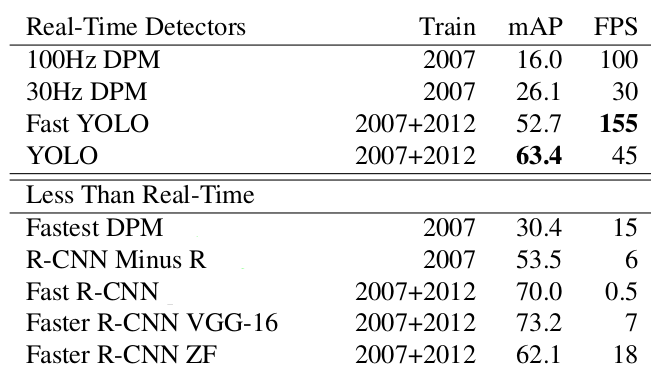
\includegraphics[width=0.8\linewidth]{test.png}
	\end{center}
	\caption{Real-Time Systems on P ASCAL VOC 2007.Compar-
		ing the performance and speed of fast detectors. Fast YOLO is
		the fastest detector on record for P ASCAL VOC detection and is
		still twice as accurate as any other real-time detector. YOLO is
		10 mAP more accurate than the fast version while still well above
		real-time in speed.}
	\label{fig:lxsfvgong}
	
	Figure\ref{fig:lxsfvgong} shows the most famous network on image classification. The accuracy and the speed is shown on the table.
	
\end{figure}


%\section{Application}

\section{conclusion}

In this paper we have discussed about the different types of image classification techniques. So this paper will help us in selecting an appropriate classification technique among all the available techniques.


\newpage
{\small
\bibliographystyle{ieee}
\bibliography{egbib}
}

\end{document}
